\documentclass{article}
\usepackage[letterpaper, margin = 1in]{geometry}
\usepackage{graphicx}
\graphicspath{.}
\usepackage{float}

\begin{document}

\noindent \textbf{Camber Effects} \\ \\
In the following simulations, the effect of camber on the produced lift spectrum is studied. As was with the previous cases, a vortex of strength $\Gamma$ = -0.02 was started upstream at an initial position of (-4.5, 0.06). While there are no analytical functions that allow us to compare the effects of camber on the lift spectrum, previous work by Martinez [1] provide some sort of comparison for trend prediction. 

\begin{figure}[h]
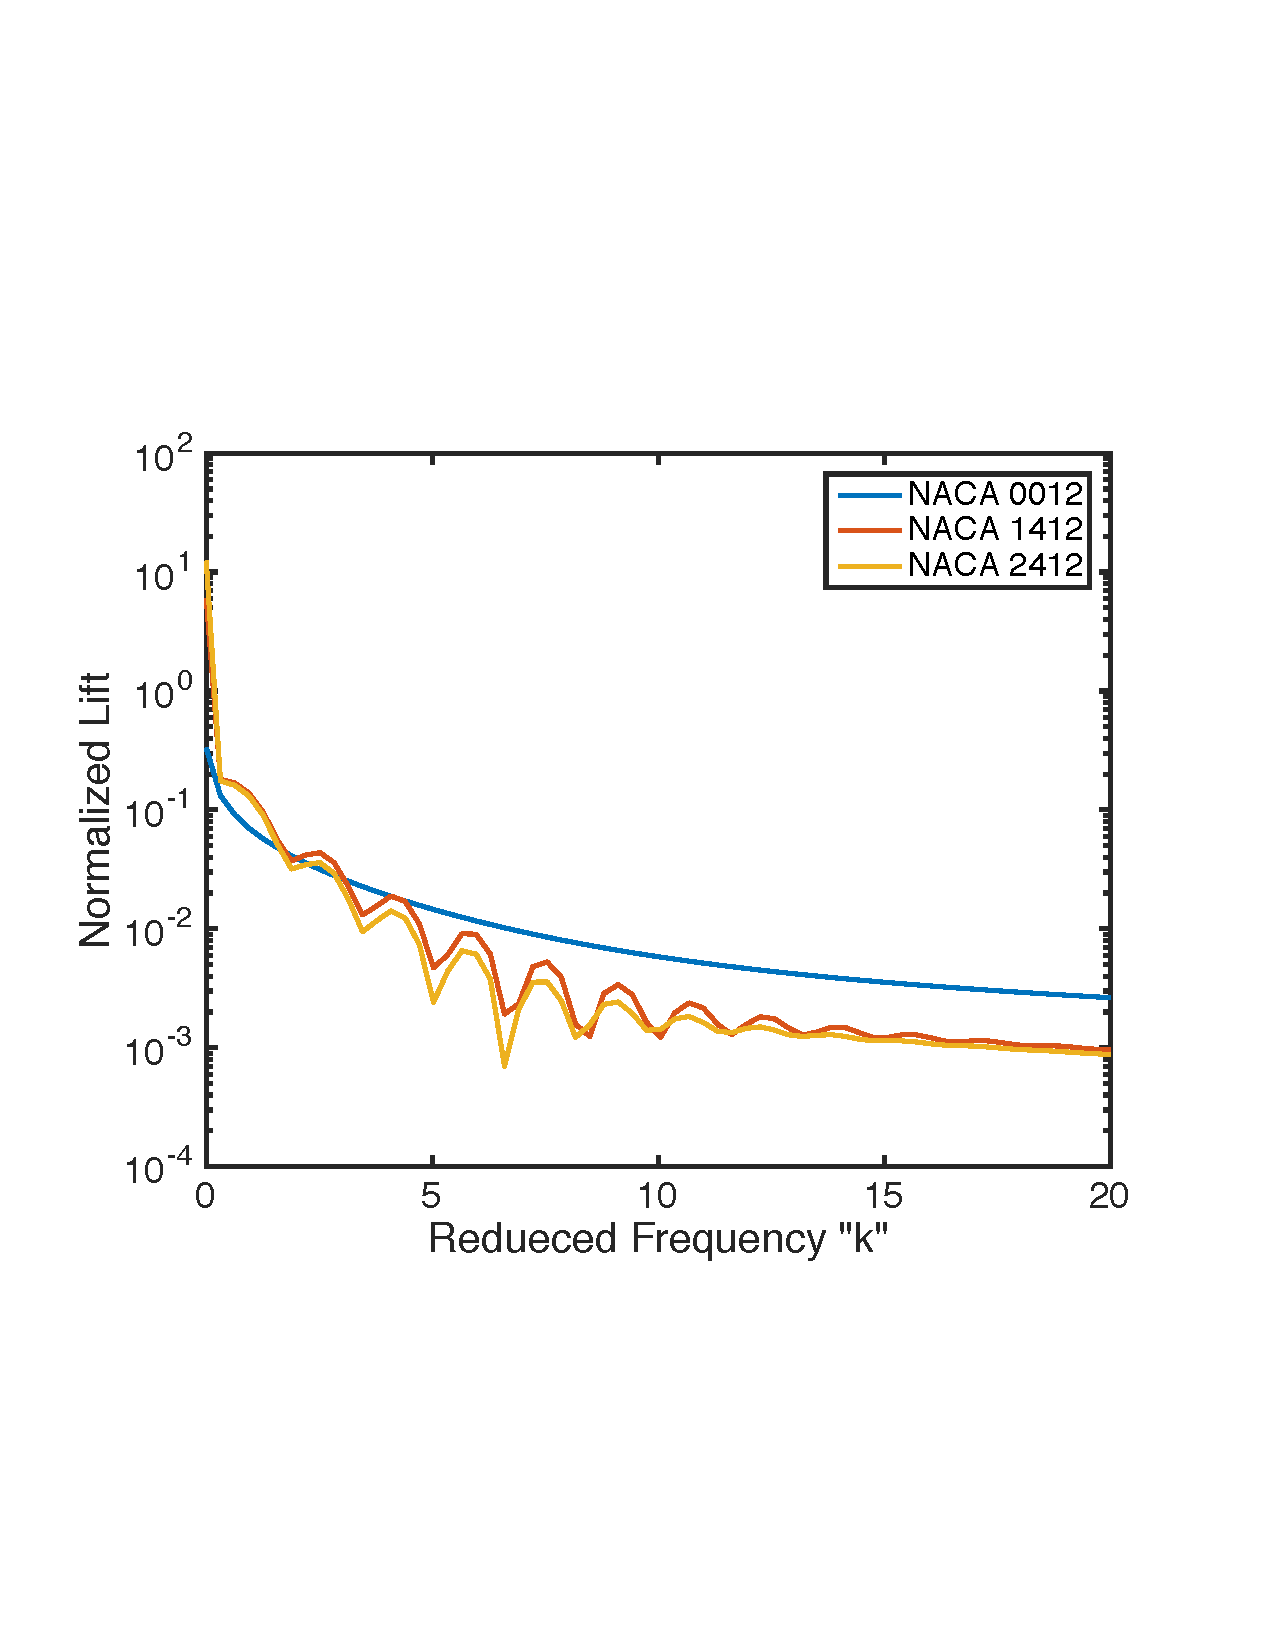
\includegraphics[width = 4in, height = 3 in]{Camber_Compare}
\centering
\caption{Effect of Camber on Lift Spectrum}
\end{figure}

\begin{figure}[h]
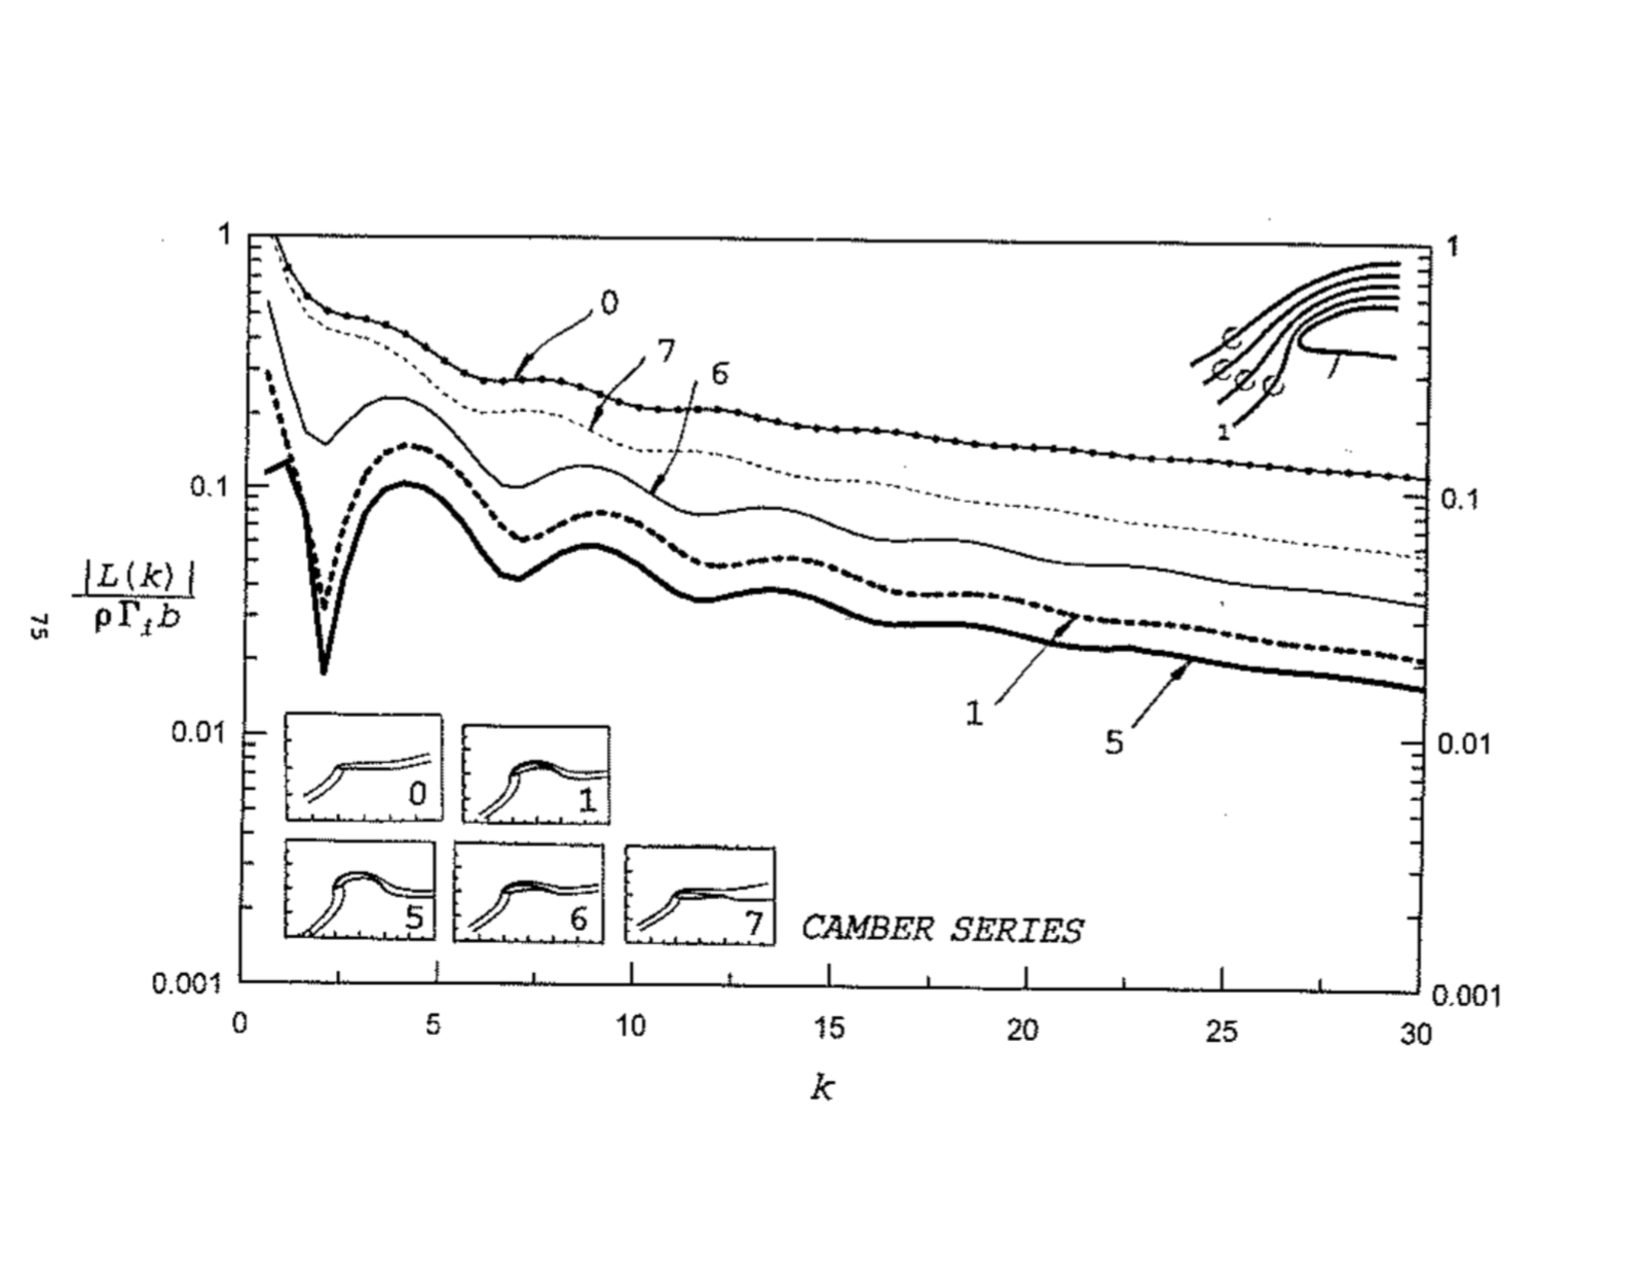
\includegraphics[width = 4in, height = 2.5 in]{Martinez_Camber}
\centering
\caption{Results of Martinez [1] showing effects of camber}
\end{figure}

\noindent Comparing the two figures, the predicted response values for the current method are smaller than those predicted in [1]. The pattern though seems to be the same with increasing camber of the airfoils resulting in a progressively smaller response. \\


[1] Martinez  R.   Rudzinsky  J.   and Atassi  H.  M.    Analytic Evaluation of Shape Effects on Blade Vortex Interaction  Dec.  1997.









\end{document}